\documentclass[../../Thesis.tex]{subfiles}
\begin{document}
\header{Research results}
\subheader{Ranking}
The figures~\ref{figure:titleRanks} \&~\ref{figure:abstractRanks} show the result of the categorization task as ranking results. The rank indicates the position of the correct journal in the sorted list of matched journals. Figure~\ref{figure:titleRanks} shows the ranking results for the different sets based on the title. Figure~\ref{figure:abstractRanks} displays the ranking results based on the abstract. Both graphs show both average and median ranks, based on the cosine-similarity between the article and journal embeddings or feature vectors.\\
\begin{figure}[hbt]
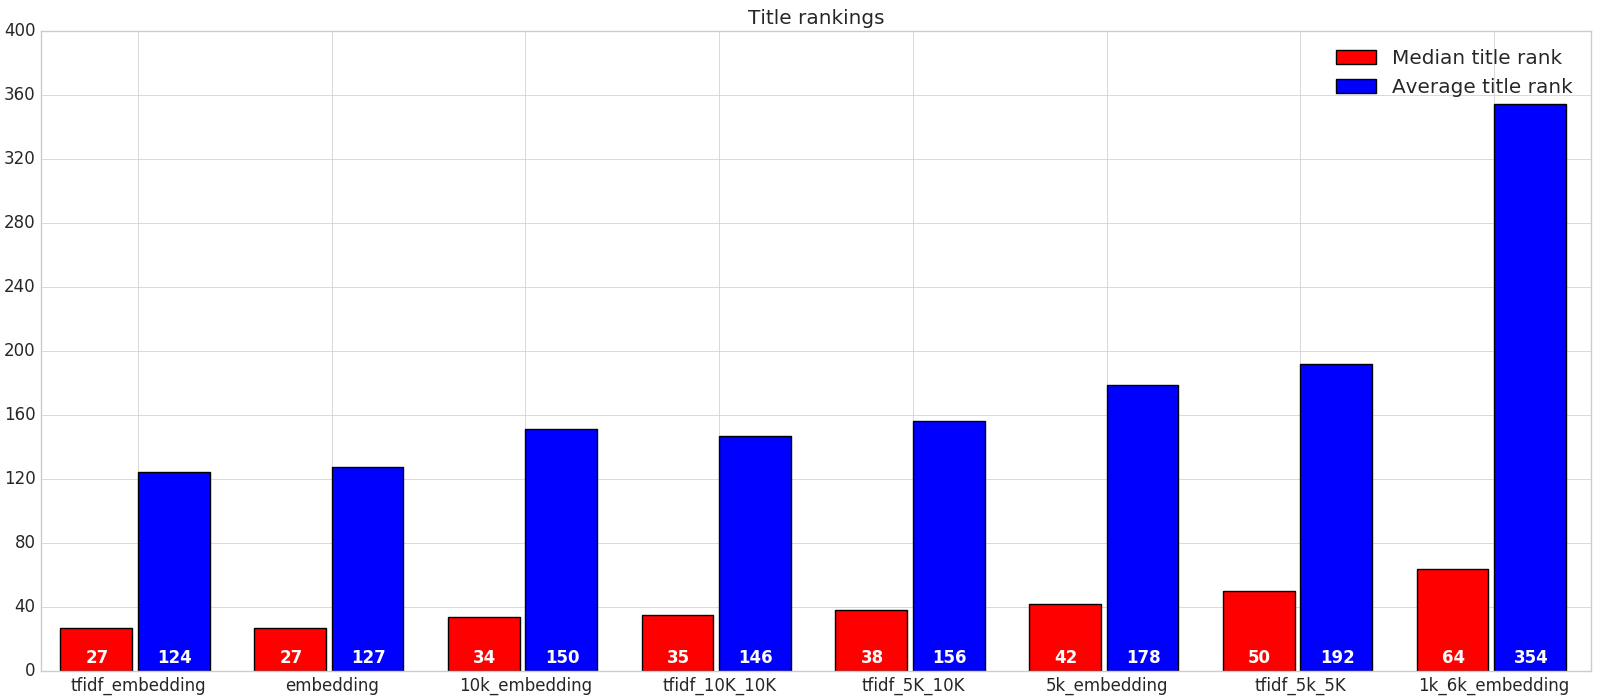
\includegraphics[width=6.5in]{Plots/Title_rankings}
\caption{Median and average title rankings}\label{figure:titleRanks}
\end{figure}
\begin{figure}[hbt]
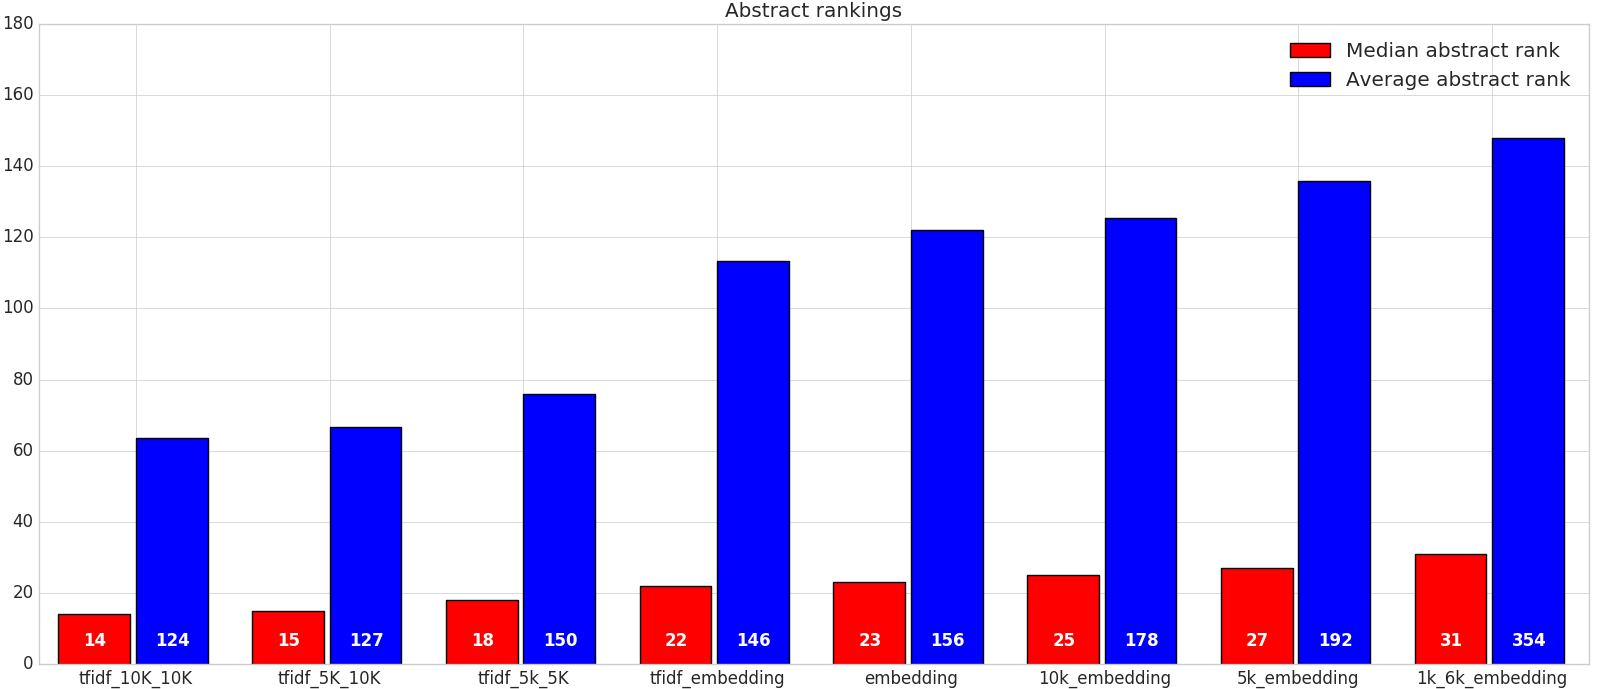
\includegraphics[width=6.5in]{Plots/Abstract_rankings}
\caption{Median and average abstract rankings}\label{figure:abstractRanks}
\end{figure}
\clearpage
\subheader{Rank distribution}
Figures~\ref{figure:titleDistribution} \&~\ref{figure:abstractDistribution} show the distributions of the ranks for each set. The figures plot the summed amount of articles against the ranks on a logarithmic scale. Figure~\ref{figure:titleDistribution} shows the rank distribution for the titles, figure~\ref{figure:abstractDistribution} shows this for the ranks based on the abstract. These graphs give a detailed view of the ranks presented in their respective figures~\ref{figure:titleRanks} \&~\ref{figure:abstractRanks}.
\begin{figure}[hbt]
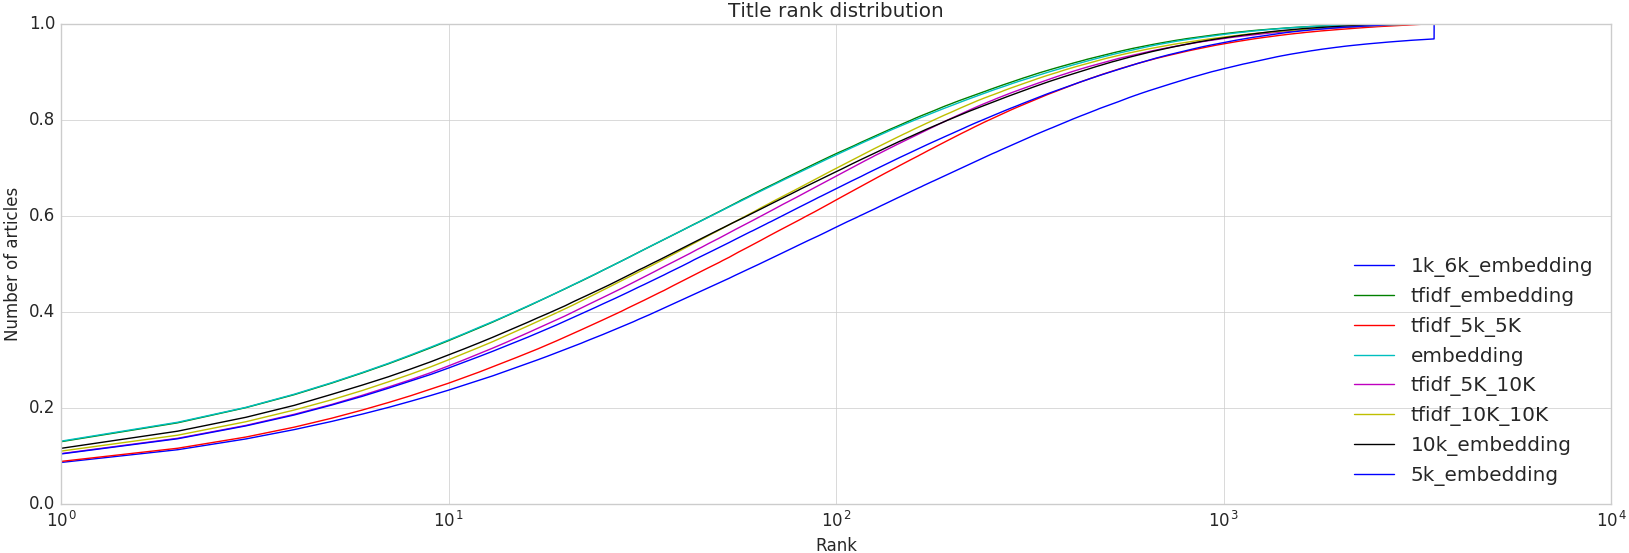
\includegraphics[width=6.5in]{Plots/Title_rank_distribution}
\caption{Title rank distribution per set}\label{figure:titleDistribution}
\end{figure}
\begin{figure}[hbt]
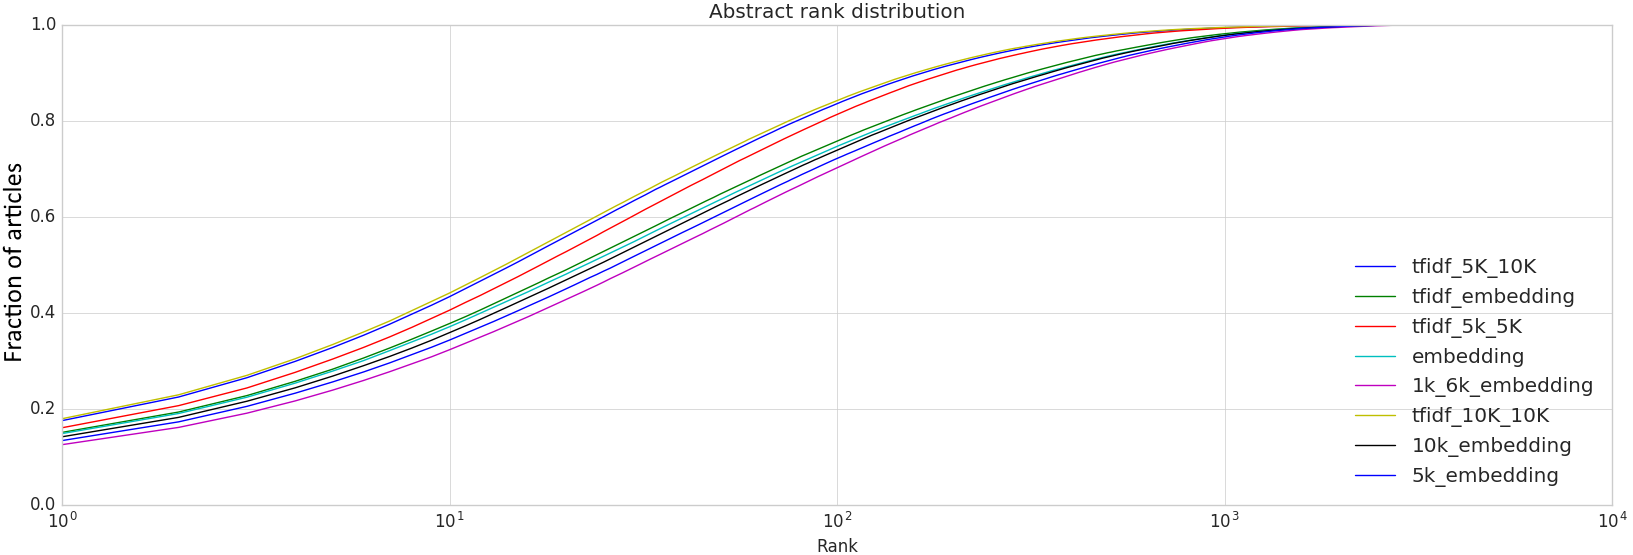
\includegraphics[width=6.5in]{Plots/Abstract_rank_distribution}
\caption{Abstract rank distribution per set}\label{figure:abstractDistribution}
\end{figure}

\clearpage
\subheader{F1-Score}
Figures~\ref{figure:f1Title} \&~\ref{figure:f1Abstract} show the precision, recall and f1 scores. These scores are calculated on journal level, and are averaged per set. Figure~\ref{figure:f1Title} shows the F1 score for the title and figure~\ref{figure:f1Abstract} shows the scores for the abstract. These scores indicate the performance of the sets on absolute hits/top-1.
\begin{figure}[hbt]
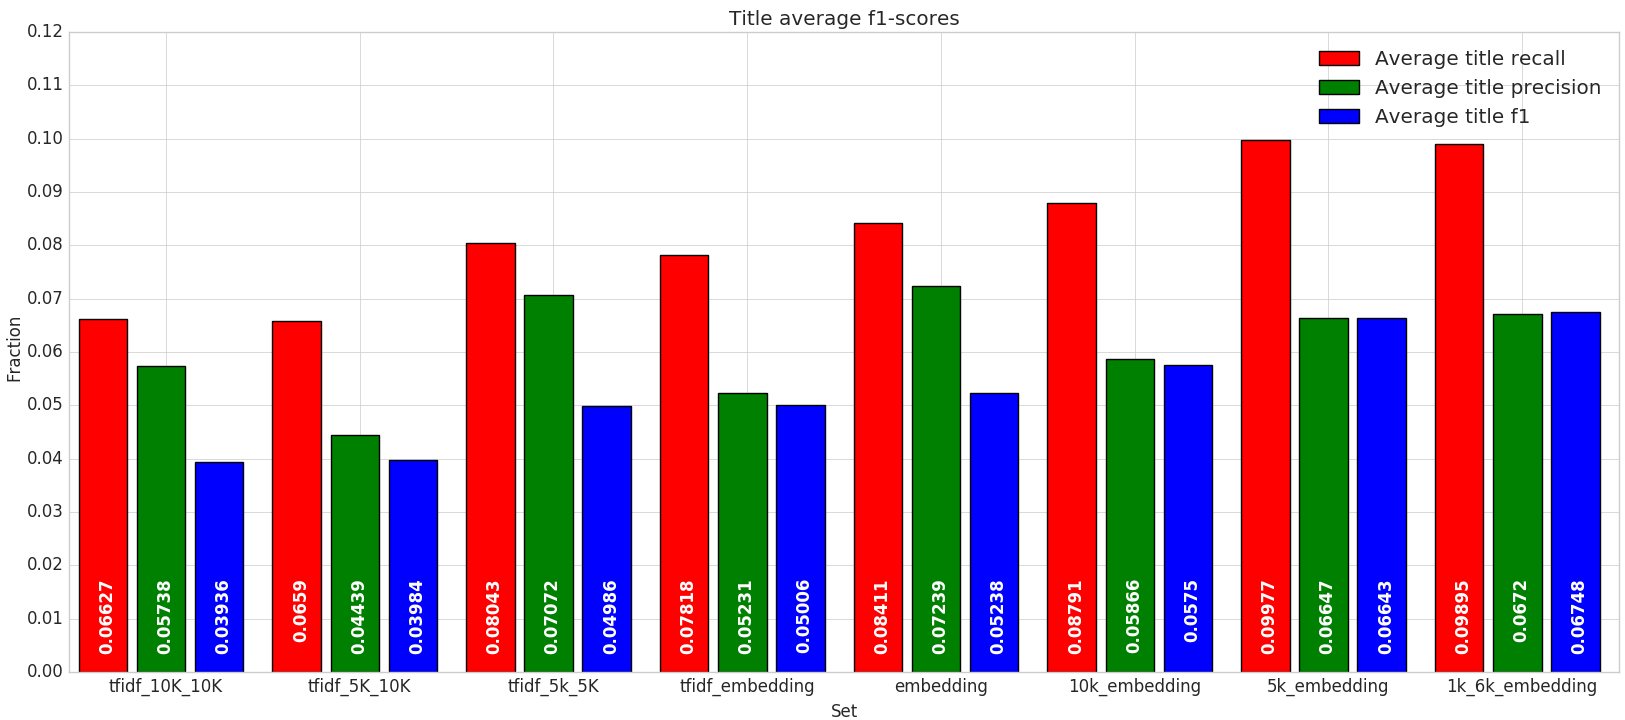
\includegraphics[width=6.5in]{Plots/Title_avg_f1}
\caption{Precision, recall and F1 scores based on title}\label{figure:f1Title}
\end{figure}
\begin{figure}[htb]
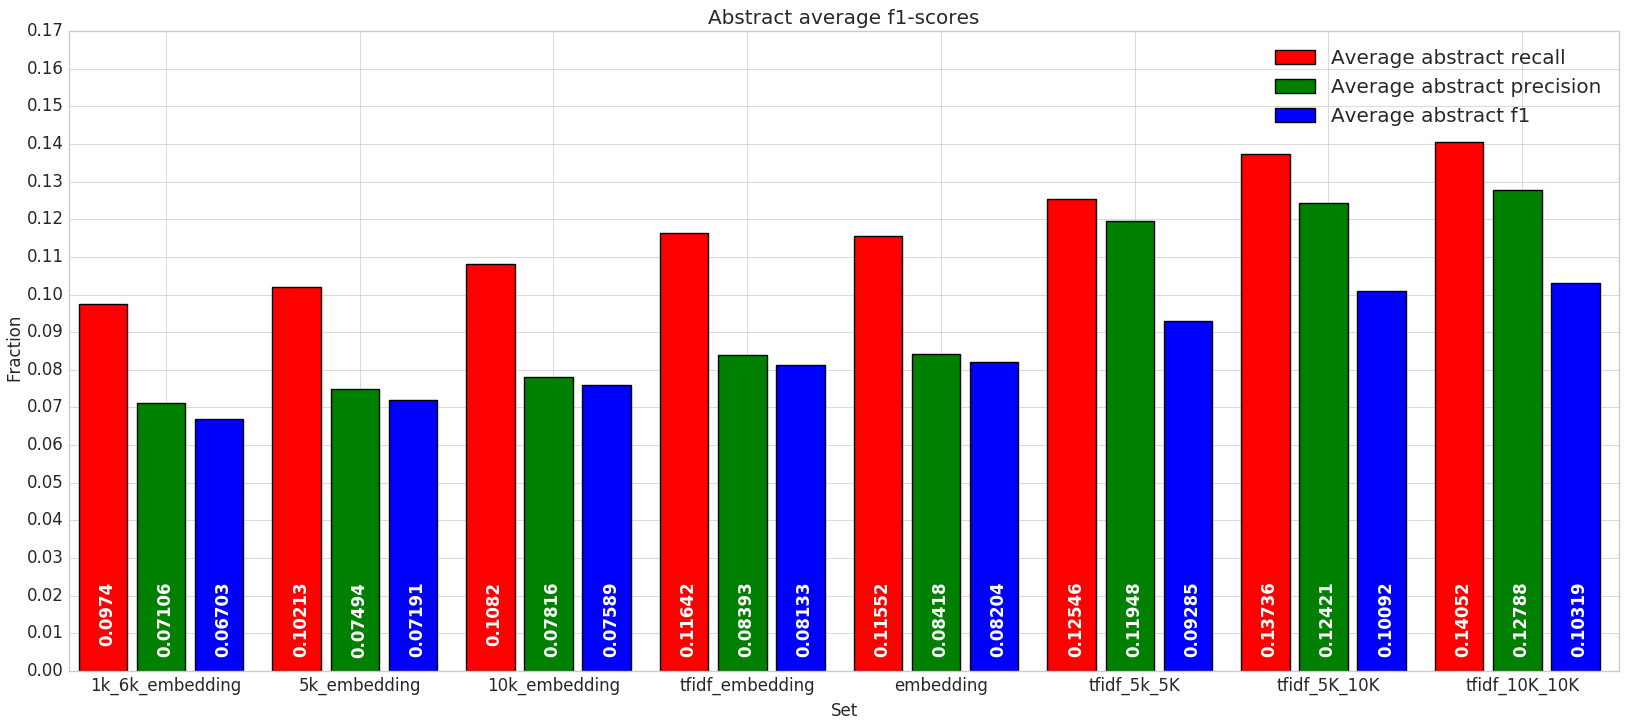
\includegraphics[width=6.5in]{Plots/Abstract_avg_f1}
\caption{Precision, recall and F1 scores based on abstract}\label{figure:f1Abstract}
\end{figure}
\clearpage
\subheader{Memory usage}
Table~\ref{table:memoryUsage} shows the total memory usage of each set for the \textit{Validation set}, indicating their storage costs in gigabytes\footnote{1024 based}.\\
\begin{table}[hbt]
\begin{center}
\begin{tabular}{|l|l|l|l|l|}
\hline
Set & Size in GB & Absolute hit percentage & Median title rank & Median abstract rank\\
&&\begin{tabular}{p{0.5in}|p{0.5in}}Title & Abstract\end{tabular}&&\\
\hline
tfidf 5k 5K & $9.82$ & \begin{tabular}{p{0.5in}|p{0.5in}}5.42\% & 10.18\%\end{tabular} & 50 & 27\\
\hline
tfidf 5K 10K & $11.47$ & \begin{tabular}{p{0.5in}|p{0.5in}}6.49\% & 11.08\%\end{tabular} & 38 & 15\\
\hline
\textbf{tfidf 10K 10K} &\textbf{11.61}& \begin{tabular}{p{0.5in}|p{0.5in}}\textbf{6.79\%} & \textbf{11.32\%}\end{tabular} & \textbf{35} & \textbf{14}\\
\hline
embedding & $3.13$ & \begin{tabular}{p{0.5in}|p{0.5in}}7.92\% & 9.24\%\end{tabular} & 27 & 23\\
\hline
5k embedding & $3.13$ & \begin{tabular}{p{0.5in}|p{0.5in}}6.34\% & 8.36\%\end{tabular} & 42 & 27\\
\hline
10k embedding & $3.13$ & \begin{tabular}{p{0.5in}|p{0.5in}}7.03\% & 8.76\%\end{tabular} & 34 & 25\\
\hline
\textbf{tfidf embedding} & \textbf{3.13} & \begin{tabular}{p{0.5in}|p{0.5in}}\textbf{7.89\%} & \textbf{9.33\%}\end{tabular} & \textbf{27} & \textbf{22}\\
\hline
1k 6k embedding & $3.06$ & \begin{tabular}{p{0.5in}|p{0.5in}}5.16\% & 7.86\%\end{tabular} & 64 &31 \\
\hline
\end{tabular}
\end{center}
\caption{Memory usage and performance for each set}\label{table:memoryUsage}
\end{table}

\end{document}


%1k_6k_embedding
%  7.85534550616

%tfidf_embedding
%  9.33435128732

%tfidf_5k_5K
%  10.1820853794

%embedding
%  9.24083300477

%tfidf_5K_10K
%  11.0842682533

%tfidf_10K_10K
%  11.3222696154

%10k_embedding
%  8.75583800194

%5k_embedding
%  8.36120161582
